\section{Chapter 5: Direct and Semidirect Products and Abelian Groups} \label{chap5}

\subsection{Direct Products} \label{sec5.1}

\defi The \textbf{direct product} of groups $G_1, G_2, \ldots, G_n$ with operations $\star_1, \star_2, \ldots, \star_n$ is the Cartesian product $G_1 \times G_2 \times \cdots \times G_n$ with the operation $\star$ defined by
\[(g_1, g_2, \ldots, g_n) \star (h_1, h_2, \ldots, h_n) = (g_1 \star_1 h_1, g_2 \star_2 h_2, \ldots, g_n \star_n h_n).\]
We may extend this to a direct product of infinitely many groups $G_1, G_2, \ldots$ with operation $\star_1, \star_2, \ldots$ whose elements are sequences $(g_1, g_2, \ldots)$.

\prop[Direct Group is a Group] \label{prop5.1}
The direct product of groups $G_1, \ldots, G_n$ is a group with order $|G_1||G_2| \cdots |G_n|$.
\begin{proof}
    To show $G = G_1 \times G_2 \cdots \times G_n$ is a group follows from the fact that each $G_i$ is a group. The identity of $G$ is $(1_1, 1_2, \ldots, 1_n)$ where $1_i \in G_i$ is the identity. The inverse of $(g_1, g_2, \ldots, g_n) \in G$ is $(g_1\inv, g_2\inv, \ldots, g_n\inv)$ where $g_i\inv \in G_i$ is the inverse of $g_i$. The order of $G$ is clear.
\end{proof}

\prop[Projections Onto Direct Groups] \label{prop5.2}
Let $G_1, \ldots, G_n$ be groups with their direct product $G$.
\begin{enumerate}
    \item Fix some $i$. Then
    \[G_i \cong \set{(1, \ldots, 1, g_i, 1, \ldots, 1) \mid g_i \in G_i} \leq G.\]
    Moreover, identifying that subgroup with $G_i$, we have $G_i \nsub G$, and
    \[G/G_i \cong G_1 \times \cdots \times G_{i-1} \times G_{i+1} \times \cdots \times G_n.\]
    \item Define $\pi_i : G \to G_i$ by $\pi_i(g_1, \ldots, g_n) = g_i$. Then $\pi_i$ is a surjective homomorphism with kernel
    \[\ker(\pi_i) = G_1 \times \cdots \times G_{i-1} \times 1 \times G_{i+1} \times \cdots \times G_n.\]
    \item If $g \in G_i$ and $h \in G_j$ for $i \neq j$, then $gh = hg$ in $G$.
\end{enumerate}

\begin{proofnum}
    \item Consider the homomorphism 
    \[\phi : G \to G_1 \times \cdots \times G_{i - 1} \times G_{i + 1} \times \cdots \times G_n, \quad \phi(g_1, \ldots, g_n) = (g_1, \ldots, g_{i - 1}, g_{i + 1}, \ldots, g_n).\] 
    It is easy to see $\ker\phi = \set{(1, \ldots, 1, g_i, 1, \ldots, 1) \mid g_i \in G_i}$ and $\phi$ is surjective. By the First Isomorphism Theorem, (i) is fully proved.
    \item Trivial.
    \item The nonidentity parts of $g$ and $h$ are in different coordinates, so they commute.
\end{proofnum}

\note For $g_i \in G_i$ and $k \in \z$, we have $(g_1g_2\cdots g_n)^k = g_1^kg_2^k \cdots g_n^k$ by \autoref{prop5.2} (iii). Hence,
\[|g_1g_2\cdots g_n| = \lcm(|g_1|, |g_2|, \ldots, |g_n|).\]

\defi The \textbf{elementary abelian} group of order $p^n$ for prime $p$ is the group
\[E_{p^n} = \underbrace{Z_p \times Z_p \times \cdots \times Z_p}_{n \text{ times}}.\]

\subsection{The Fundamental Theorem of Finitely Generated Abelian Groups}

\defi $G$ is \textbf{finitely generated} if some finite $A \subset G$ exists such that $G = \gen A$.

\defi The \textbf{free abelian group of rank $r$} is the direct product of $r$ copies of $\z$, denoted $\z^r$, with $\z^0 = 1$. Moreover, $\z^r = \gen A$, where $A = \set{e_1, e_2, \ldots, e_r}$ and each $e_i$ is the standard basis vector with $1$ in the $i$-th coordinate and $0$ in all other coordinates.

\theo[Fundamental Theorem of Finitely Generated Abelian Groups] \label{theo5.3}
Let $G$ be a finitely generated abelian group. Then
\begin{enumerate}
    \item 
    \[G \cong \z^r \times Z_{n_1} \times Z_{n_2} \times \cdots \times Z_{n_s},\]
    for integers $r, n_1, n_2, \ldots, n_s$ satisfying:
    \begin{enumerate}
        \item $r \geq 0, n_j \geq 2$ for all $j$, and
        \item $n_{i + 1} \mid n_i$ for $1 \leq i \leq s - 1$.
    \end{enumerate}
    \item The expression in (i) is unique: if $G \cong \z^u \times Z_{m_1} \times Z_{m_2} \times \cdots \times Z_{m_v}$ for integers $u, m_1, m_2, \ldots, m_v$ satisfying the same conditions as in (i), then $r = u$, $s = v$, and $n_i = m_i$ for all $i$.
\end{enumerate}

\begin{proof}
    Derived in \autoref{sec12.1} as a consequence of a more general classification theorem. An alternate proof for finite groups is given at the end of \autoref{sec6.1}.
\end{proof}

\defi With respect to \autoref{theo5.3}:
\begin{itemize}
    \item The number $r$ is the \textbf{free rank} or \textbf{Betti number} of $G$,
    \item the integers $n_i$ are the \textbf{invariant factors} of $G$, and
    \item the expression of $G$ is the \textbf{invariant factor decomposition} of $G$.
\end{itemize}

\defi If $G$ is finite abelian with invariant factors $n_1, n_2, \ldots, n_s$, then $G$ is of \textbf{type} $(n_1, n_2, \ldots, n_s)$.

\note For some $G$ with type $(n_1, n_2, \ldots, n_s)$, then all $n_i \mid n_1$. In particular, square free orders imply that $G$ is cyclic, as in \autoref{cor5.4}:

\cor[Squarefree Order is Unique Abelian Group] \label{cor5.4}
If $n$ is squarefree, then the only abelian group of order $n$ is the cyclic group $Z_n$, up to isomorphism.

\begin{proof}
    Squarefree order implies $G$ has type $n_1 = n$ and $n_j = 1$ for all other $j$, hence $G \cong Z_n$.
\end{proof}

\ex We have $180 = 2^2 \cdot 3^2 \cdot 5$. Note that $2 \cdot 3 \cdot 5 \mid n_1$, so the only choices for $n_1$ are $2^2 \cdot 3^2 \cdot 5$, $2^2 \cdot 3 \cdot 5$, $2 \cdot 3^2 \cdot 5$, and $2 \cdot 3 \cdot 5$. For each choice, we construct potential $n_2$ with $n_2 \mid n_1$ and $n_1n_2 \mid n$. Similarly, we may choose $n_3$ with $n_3 \mid n_2$ and $n_1n_2n_3 \mid n$. We get the following list of sequences:
\begin{itemize}
    \item $n_1 = 2^2 \cdot 3^2 \cdot 5$, $n_2 = 1$, $n_3 = 1$ corresponds to $Z_{180}$.
    \item $n_1 = 2 \cdot 3^2 \cdot 5$, $n_2 = 2$, $n_3 = 1$ corresponds to $Z_{90} \times Z_2$.
    \item $n_1 = 2^2 \cdot 3 \cdot 5$, $n_2 = 3$, $n_3 = 1$ corresponds to $Z_{60} \times Z_3$.
    \item $n_1 = 2 \cdot 3 \cdot 5$, $n_2 = 6$, $n_3 = 1$ corresponds to $Z_{30} \times Z_6$.
\end{itemize}

\theo[Primary Decomposition Theorem for Finite Abelian Groups] \label{theo5.5}
Let $G$ be abelian with order $n$ that has prime factorization $n = p_1^{\alpha_1} p_2^{\alpha_2} \cdots p_k^{\alpha_k}$. Then
\begin{enumerate}
    \item $G \cong H_1 \times H_2 \times \cdots \times H_k$ where $|H_i| = p_i^{\alpha_i}$,
    \item for each $H \in \set{H_1, H_2, \ldots, H_k}$ with $|H| = p^\alpha$, then
    \[H \cong Z_{p^{\beta_1}} \times Z_{p^{\beta_2}} \times \cdots \times Z_{p^{\beta_m}}\]
    where $\beta_1, \beta_2, \ldots, \beta_m$ form a partition of $\alpha$ such that $\beta_{i + 1} \leq \beta_i$ for $1 \leq i \leq m - 1$, and
    \item the decomposition in (i) and (ii) is unique: if $G \cong K_1 \times K_2 \times \cdots \times K_r$ with $|K_i| = p_i^{\alpha_i}$ for all $i$, then $H_i \cong K_i$, and they have the same invariant factors.
\end{enumerate}

\begin{proof}
    Proven later.
\end{proof}

\defi With respect to \autoref{theo5.5}:
\begin{itemize}
    \item The integers \smash{$p_i^{\beta_j}$} are the \textbf{elementary divisors} of $G$, and
    \item the expression of $G$ in (ii) is the \textbf{elementary divisor decomposition} of $G$.
\end{itemize}

\note If $G$ is a $p$-group, say $|G| = p^\alpha$, then the number of nonisomorphic abelian groups of order $p^\alpha$ is the number of partitions of $\alpha$. Hence, the number of nonisomorphic abelian groups of order $n = p_1^{\alpha_1} p_2^{\alpha_2} \cdots p_k^{\alpha_k}$ with $q_i$ representing the number of partitions of $\alpha_i$ is $q_1q_2 \cdots q_k$.

\ex Suppose $n = 1800 = 2^3 \cdot 3^2 \cdot 5^2$. Then we have
\[
\begin{array}{c|c|c}
    \text{Order $p^\beta$} & \text{Partitions of $\beta$} & \text{Abelian Groups} \\
    \hline
    2^3 & 3; \quad 2, 1; \quad 1, 1, 1 & Z_{8}, \, Z_4 \times Z_2, \, Z_2 \times Z_2 \times Z_2 \\
    3^2 & 2; \quad 1, 1 & Z_9, \, Z_3 \times Z_3 \\
    5^2 & 2; \quad 1, 1 & Z_{25}, \, Z_5 \times Z_5
\end{array}\]
Then we have a total of 12 potential isomorphism types by taking all possible direct products from each abelian group of order $2^3$, $3^2$, and $5^2$:
\[
\begin{array}{ll}
    Z_8 \times Z_9 \times Z_{25} & Z_4 \times Z_2 \times Z_3 \times Z_3 \times Z_{25} \\
    Z_8 \times Z_9 \times Z_5 \times Z_5 & Z_4 \times Z_2 \times Z_3 \times Z_3 \times Z_5 \times Z_5 \\
    Z_8 \times Z_3 \times Z_3 \times Z_{25} & Z_2 \times Z_2 \times Z_2 \times Z_9 \times Z_{25} \\
    Z_8 \times Z_3 \times Z_3 \times Z_5 \times Z_5 & Z_2 \times Z_2 \times Z_2 \times Z_9 \times Z_5 \times Z_5 \\
    Z_4 \times Z_2 \times Z_9 \times Z_{25} & Z_2 \times Z_2 \times Z_2 \times Z_3 \times Z_3 \times Z_{25} \\
    Z_4 \times Z_2 \times Z_9 \times Z_5 \times Z_5 & Z_2 \times Z_2 \times Z_2 \times Z_3 \times Z_3 \times Z_5 \times Z_5
\end{array}\]

\prop[Cyclic Decomposition Criterion] \label{prop5.6}
Let $m, n \in \zp$.
\begin{enumerate}
    \item $Z_m \times Z_n \cong Z_{mn}$ if and only if $(m, n) = 1$, and
    \item if $n = p_1^{\alpha_1} p_2^{\alpha_2} \cdots p_k^{\alpha_k}$, then $Z_n \cong Z_{p_1^{\alpha_1}} \times Z_{p_2^{\alpha_2}} \times \cdots \times Z_{p_k^{\alpha_k}}$.
\end{enumerate}

\begin{proofnum}
    \item Put $Z_m = \gen g, Z_n = \gen h$, and $\ell = \lcm(m, n)$. Recall from \autoref{sec0.2} that $\lcm(m, n) = mn$ if and only if $(m, n) = 1$. Let $g^sh^t \in Z_m \times Z_n$, Then $(g^sh^t)^\ell = g^{s\ell}h^{t\ell} = 1$. If $(m, n) \neq 1$, every element would be strictly less than $mn$, hence $Z_m \times Z_n \not\cong Z_{mn}$.
    
    If $(m, n) = 1$ instead, then $|gh| = mn$. The result is clear.
    \item Follows from (i) using induction on $k$.
\end{proofnum}

\note Let $G$ be abelian of type $(n_1, n_2, \ldots, n_k)$. Let $n = p_1^{\alpha_1} p_2^{\alpha_2} \cdots p_m^{\alpha_m} = n_1n_2 \cdots n_k$. Put each $n_i$ as
\[n_i = p_1^{\beta_{i1}} p_2^{\beta_{i2}} \cdots p_m^{\beta_{im}}\]
where $\beta_{ij} \geq 0$ for all $i, j$. Then by \autoref{prop5.6}, we have
\[Z_{n_i} \cong Z_{p_1^{\beta_{i1}}} \times Z_{p_2^{\beta_{i2}}} \times \cdots \times Z_{p_m^{\beta_{im}}}.\]
Then the elementary divisors of $G$ are the integers $p_j^{\beta_{ij}}$ for $1 \leq i \leq k$ and $1 \leq j \leq m$ such that $\beta_{ij} > 0$.

We may also collect all $Z_{p_j^{\beta_{ij}}}$ for $1 \leq i \leq k$ to obtain the Sylow $p_j$-subgroup of $G$.

\ex If $|G| = 1800 = 2^3 \cdot 3^2 \cdot 5^2$ of type $(30, 30, 2)$, observe that $Z_{30} \cong Z_2 \times Z_3 \times Z_5$. Then
\[G \cong Z_{30} \times Z_{30} \times Z_2 \cong Z_2 \times Z_3 \times Z_5 \times Z_2 \times Z_3 \times Z_5 \times Z_2,\]
and $P \in \syl_2(G)$ is isomorphic to $Z_2 \times Z_2 \times Z_2$, $Q \in \syl_3(G)$ is isomorphic to $Z_3 \times Z_3$, and $R \in \syl_5(G)$ is isomorphic to $Z_5 \times Z_5$. Hence, the elementary divisors of $G$ are $2, 2, 2, 3, 3, 5, 5$.

\note If $G$ is a direct product of cyclic groups, the above process may be performed to obtain the elementary divisors of $G$.

\ex Consider the following calculations:
\begin{enumerate}
    \item $G = Z_6 \times Z_{15} \cong Z_2 \times Z_3 \times Z_3 \times Z_5$ has elementary divisors $2, 3, 3, 5$.
    \item $G = Z_{21} \times Z_6 \times Z_{15} \cong Z_3 \times Z_7 \times Z_2 \times Z_3 \times Z_3 \times Z_5$ has elementary divisors $2, 3, 3, 3, 5, 7$.
    \item $G = Z_{22} \times Z_{42} \cong Z_2 \times Z_{11} \times Z_2 \times Z_3 \times Z_7$ has elementary divisors $2, 2, 3, 7, 11$.
\end{enumerate}

\newpage

\ex Let $G$ be an abelian group of order $n = p_1^{\alpha_1} p_2^{\alpha_2} \cdots p_k^{\alpha_k}$ with a given list of elementary divisors. To find the invariant factors of $G$, we follow the following steps:
\begin{enumerate}
    \item Group the elementary divisors that are powers of the same prime together. We then obtain $k$ lists of integers, one for each prime $p_j$.
    \item Arrange the integers in nondecreasing order in each list.
    \item Among the $k$ lists, suppose that the longest (the one with the most terms) consists of $t$ integers. If a list has fewer than $t$ integers, then we append $1$'s to the end of the list until it has $t$ integers. We then have $k$ lists of $t$ integers.
    \item For each $i \in \set{1, 2, \ldots, t}$, we multiply the $i$-th integers from each of the $k$ lists together to obtain $n_i$. We then have a list of $t$ integers $n_1, n_2, \ldots, n_t$.
\end{enumerate}

Note that the ordering of these lists is structured in such a way to ensure divisibility of the invariant factors. As an example, take $G$ with elementary divisors $2, 3, 2, 25, 3, 2$. We then regroup the elementary divisors into lists of powers of the same prime:
\[
\begin{array}{c|c|c}
    p = 2 & p = 3 & p = 5 \\
    \hline
    2 & 3 & 25 \\
    2 & 3 & 1 \\
    2 & 1 & 1
\end{array}\]
We then multiply the integers in each row together to obtain the invariant factors $n_1 = 2 \cdot 3 \cdot 25$, $n_2 = 2 \cdot 3 \cdot 1$, and $n_3 = 2 \cdot 1 \cdot 1$. Hence, the invariant factor decomposition of $G$ is
\[G \cong Z_{150} \times Z_6 \times Z_2\]
Refer to the previous list of the 12 abelian groups of order 1800 to see that this is indeed one of the groups:
\[
\begin{array}{ll}
    Z_{1800} & Z_{300} \times Z_6 \\
    Z_{360} \times Z_5 & Z_{60} \times Z_{30} \\
    Z_{600} \times Z_3 & Z_{450} \times Z_2 \times Z_2 \\
    Z_{120} \times Z_{15} & Z_{90} \times Z_{10} \times Z_2 \\
    Z_{900} \times Z_2 & Z_{150} \times Z_6 \times Z_2 \\
    Z_{180} \times Z_{10} & Z_{30} \times Z_{30} \times Z_2
\end{array}\]

\newpage

\subsection{Table of Groups of Small Order}

\defi The group $Z_3 \semidir Z_4$ is the group of order 12 with presentation
\[\gen{x, y \mid x^3 = y^4 = 1, xyx\inv = y^2},\]
and $\gen y \in \syl_3(Z_3 \semidir Z_4)$ is inverted by $x$ acting by conjugation.

\defi The group $(Z_3 \times Z_3) \semidir Z_2$ is the group of order 18 with presentation
\[\gen{x, y, z \mid x^2 = y^3 = z^3 = 1, yz = zy, x\inv yx = y\inv, x\inv zx = z\inv},\]
and $\gen{y, z} \in \syl_3((Z_3 \times Z_3) \semidir Z_2)$ is inverted by $x$ acting by conjugation.

\defi The group $Z_5 \semidir Z_4$ is the group of order 20 with presentation
\[\gen{x, y \mid x^4 = y^5 = 1, x\inv yx = y\inv},\]
and $\gen y \in \syl_5(Z_5 \semidir Z_4)$ is inverted by $x$ acting by conjugation.

\defi The \textbf{Frobenius group} of order 20 is the group $F_{20}$ with presentation
\[\gen{x, y \mid x^4 = y^5 = 1, x\inv yx = y^2},\]
and $\gen y \in \syl_5(F_{20})$ is inverted by $x$ acting by conjugation. This appears as the normalizer of a Sylow 5-subgroup of $S_5$, namely:
\[F_{20} = \gen{(2\ 3\ 5\ 4), (1\ 2\ 3\ 4\ 5)}.\]

\note The following table lists all abelian groups of order $n$ for $1 \leq n \leq 20$ up to isomorphism: first column is order, second column is the number of nonisomorphic groups of that order, third column is the list of abelian groups of that order, and fourth column is the list of nonabelian groups of that order.

\textit{Remark: the listed nonabelian groups of order 16 are from my own lists, which Dummit and Foote do not provide.}
\[
\begin{array}{c|c|c|c}
    n & \text{Number of Groups} & \text{Abelian Groups} & \text{Nonabelian Groups} \\
    \hline
    1 & 1 & Z_1 & - \\
    \hline
    2 & 1 & Z_2 & - \\
    \hline
    3 & 1 & Z_3 & - \\
    \hline
    4 & 2 & Z_4, V_4 & - \\
    \hline
    5 & 1 & Z_5 & - \\
    \hline
    6 & 2 & Z_6 & S_3 \\
    \hline
    7 & 1 & Z_7 & - \\
    \hline
    8 & 3 & Z_8, Z_4 \times Z_2, Z_2 \times Z_2 \times Z_2 & D_8, Q_8 \\
    \hline
    9 & 2 & Z_9, Z_3 \times Z_3 & - \\
    \hline
    10 & 2 & Z_{10} & D_{10} \\
    \hline
    11 & 1 & Z_{11} & - \\
    \hline
    12 & 5 & Z_{12}, Z_6 \times Z_2& A_4, D_{12}, Z_3 \semidir Z_4 \\
    \hline
    13 & 1 & Z_{13} & - \\
    \hline
    14 & 2 & Z_{14}, Z_{7} \times Z_{2} & D_{14} \\
    \hline
    15 & 1 & Z_{15} & - \\
    \hline
    16 & 14 & Z_{16}, Z_8 \times Z_2, Z_4 \times Z_4 & Z_4 \semidir V_4, Z_4 \semidir Z_4, M, D_{16}, QD_{16}, Q_{16} \\
    & & Z_4 \times V_4, Z_2 \times Z_2 \times Z_2 \times Z_2 & D_8 \semidir Z_2, Q_8 \semidir Z_2, D_8 * Z_4 \\
    \hline
    17 & 1 & Z_{17} & - \\
    \hline
    18 & 5 & Z_{18}, Z_6 \times Z_3 & D_{18}, S_3 \times Z_3, (Z_3 \times Z_3) \semidir Z_2 \\
    \hline
    19 & 1 & Z_{19} & - \\
    \hline
    20 & 5 & Z_{20}, Z_{10} \times Z_{2} & D_{20}, Z_5 \semidir Z_4, F_{20}
\end{array}\]

\newpage

\subsection{Recognizing Direct Products}

\defi Let $g, h \in G$ and $H, K \subseteq G$ be nonempty.
\begin{itemize}
    \item Define $[g, h] = g\inv h\inv gh$, the \textbf{commutator} of $g$ and $h$.
    \item Define $[H, K] = \gen{[h, k] \mid h \in H, k \in K}$, the subgroup generated by commutators of elements of $H$ and $K$.
    \item Define $G' = \gen{[g, h] \mid g, h \in G}$, the \textbf{commutator subgroup} of $G$.
\end{itemize}

\prop[Properties of Commutators] \label{prop5.7}
Let $g, h \in G$ and $H \leq G$. Then
\begin{enumerate}
    \item $gh = hg[g, h]$,
    \item $H \nsub G$ if and only if $[H, G] \leq H$,
    \item $\sigma[g, h] = [\sigma(g), \sigma(h)]$ for any $\sigma \in \aut(G)$, $G' \cha G$, and $G/G'$ is abelian.
    \item $G/G'$ is the largest abelian quotient of $G$ in that if $H \nsub G$ and $G/H$ is abelian, then $G' \leq H$. Conversely, $G' \leq H$ implies $H \nsub G$, and $G/H$ is abelian.
    \item If $\phi : G \to A$ is a homomorphism into $A$ abelian, then $\phi$ factors through $G'$, i.e., $G' \leq \ker\phi$, and the following diagram commutes:
    \begin{center}
        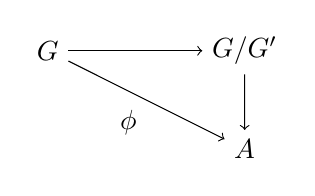
\begin{tikzpicture}[scale=1.25]
            \node (G) at (0, 0) {$G$};
            \node (GG) at (2, 0) {$G/G'$};
            \node (A) at (2, -1) {$A$};

            \draw [->] (G) -- (GG);
            \draw [->] (G) -- node [below left] {$\phi$} (A);
            \draw [->] (GG) -- (A);
        \end{tikzpicture}
    \end{center}
\end{enumerate}

\begin{proofnum}
    \item Clear.
    \item $H \nsub G \iff g\inv hg \in H \iff h\inv g\inv hg \in H \iff [h, g] \in H$ for all $g \in G$ and $h \in H$.
    \item For $\sigma \in \aut(G)$, then
    \[\sigma[g, h] = \sigma(g\inv h\inv gh) = \sigma(g)\inv \sigma(h)\inv \sigma(g)\sigma(h) = [\sigma(g), \sigma(h)].\]
    Then $\sigma[g, h] \in G'$. Invertibility of $\sigma$ implies $G' \subseteq \sigma(G')$, and hence $G' = \sigma(G')$. Then $G' \cha G$. Finally, for any $g, h \in G$, we have by (i) that
    \[(gG')(hG') = ghG' = hg[g, h]G' = hgG' = (hG')(gG'),\]
    and hence $G/G'$ is abelian.
    \item If $H \nsub G$ and $G/H$ is abelian, then for $g, h \in G$, we have
    \[1H = (gH)\inv (hH)\inv (gH)(hH) = [g, h]H,\]
    and hence $[g, h] \in H$.
    
    Conversely, $G' \leq H$ and $G/G'$ abelian by (iii) implies every subgroup of $G/G'$ is normal, and hence $H/H' \nsub G/G'$. By the Lattice Isomorphism Theorem, $H \nsub G$. By the Third Isomorphism Theorem, then
    \[G/H \cong (G/G')/(H/G'),\]
    and hence $G/H$ is abelian.
    \item Clear from (iv).
\end{proofnum}

\ex A group $G$ is abelian if and only if $G' = 1$. To see this, simply note that abelian $G$ implies $[g, h] = 1$ for every $g, h \in G$. The converse is clear from assuming trivial $G'$.

\ex Let $D_{2n}$ have usual representation. Note that $[r, s] = r^{-2}$, hence $\gen{r^{-2}} = \gen{r^2} \leq D_{2n}'$. Moreover, $\gen{r^2} \nsub D_{2n}$, since $sr^2s\inv = r^{-2} \in \gen{r^2}$. Note that $|\bar s| = |\bar r| = 2$, hence $\bar{sr} = \bar{rs}$, and $D_{2n}/\gen{r^2}$ is abelian. By \autoref{prop5.7}(iv), we have $D_{2n}' \leq \gen{r^2}$, and hence $D_{2n}' = \gen{r^2}$. If $n$ is odd, then $\gen{r^2} = \gen r$, whereas $n$ even implies $\gen{r^2}$ is of index 2 in $\gen r$. Hence, $D_{2n}'$ is of index 2 or 4 in $D_{2n}$ whether $n$ is odd or even, respectively.

\newpage

\prop[Counting Factorization in Product Subgroup] \label{prop5.8}
Let $H, K \leq G$. Then the number of distinct factorizations of $g \in HK$ as $g = hk$ with $h \in H$ and $k \in K$ is $|H \cap K|$. In particular, $H \cap K = 1$ implies each $g \in HK$ has unique factorization as $g = hk$ with $h \in H$ and $k \in K$.

\begin{proof}
    Let $g = h_0k_0 \in HK$ for some $h_0 \in H, k_0 \in K$. Then $g \in h_0K$. If $g = hk$ for some $h \in H, k \in K$, then $g \in hK$, hence $hK = h_0K$. This implies $h\inv h_0 \in K$, and since $h\inv h_0 \in H$, we have $h\inv h_0 \in H \cap K$. Set $h_0 = hx$ for some $x \in H \cap K$. Since $g = hk = h_0k_0$, we know $hk = hxk_0$, hence $k = xk_0$. Then every factorization of $g$ has the form $g = (h_0x\inv)(xk_0)$ for $x \in H \cap K$. Conversely, for any $x \in H \cap K$, we have $g = (h_0x\inv)(xk_0)$, and hence the number of distinct factorizations of $g$ is $|H \cap K|$.
\end{proof}

\theo[Direct Product Recognition Theorem] \label{theo5.9}
Let $H, K \leq G$ such that
\begin{enumerate}
    \item $H \nsub G$ and $K \nsub G$, and
    \item $H \cap K = 1$.
\end{enumerate}
Then $HK \cong H \times K$.
\begin{proof}
    We know $HK \leq G$ by \autoref{cor3.15}. Let $h \in H$ and $k \in K$. Observe $[h, k] \in H \cap K = 1$, hence $hk = kh$. By \autoref{prop5.8}, every $g \in HK$ has unique factorization as $g = hk$ with $h \in H$ and $k \in K$. Define $\phi : H \times K \to HK$ by $\phi(h, k) = hk$. This is a bijection by the uniqueness of factorization. Moreover, for $(h_1, k_1), (h_2, k_2) \in H \times K$, we have
    \[\phi((h_1, k_1)(h_2, k_2)) = \phi(h_1h_2, k_1k_2) = h_1h_2k_1k_2 = h_1k_1h_2k_2 = \phi(h_1, k_1)\phi(h_2, k_2),\]
    and hence $\phi$ is a homomorphism. Therefore, $HK \cong H \times K$.
\end{proof}

\defi Let $H \nsub G$ and $K \nsub G$ with $H \cap K = 1$. Then $HK$ is the \textbf{internal direct product} of $H$ and $K$. We call $H \times K$ the \textbf{external direct product} of $H$ and $K$.

\subsection{Semidirect Products}

\begin{defn}
    \item Let $H$ and $K$ be groups, and let $\phi : K \to \aut(H)$ be a homomorphism. The \textbf{semidirect product} of $H$ and $K$ with respect to $\phi$ is the group $H \semidir_\phi K$. If the homomorphism $\phi$ is clear from the context, then we simply write $H \semidir K$.
    \item The \textbf{generalized quaternion group of order $2^{n + 1}$} is the group
    \[Q_{2^{n + 1}} = \gen{h, x \mid h^{2^n} = x^4 = 1, x\inv hx = h\inv, h^{2^{n - 1}} = x^2}\]
    for $n \geq 2$.
    \item Let $H$ be a group with $K = \aut(H)$, and $\phi = \id$. Then the semidirect product $H \semidir_\phi K$ is called the \textbf{holomorph} of $H$, denoted $\hol(H)$.
\end{defn}

\begin{theo}[Semidirect Product Construction]
    \label{theo5.10}
    Let $H$ and $K$ be groups, and let $\phi : K \to \aut(H)$ be a homomorphism. Let $\cdot$ be the action of $K$ on $H$ determined by $\phi$. Let $G$ be the set of ordered pairs $(h, k)$ with $h \in H$ and $k \in K$ with the defined multiplication:
    \[(h_1, k_1)(h_2, k_2) = (h_1 (k_1 \cdot h_2), k_1 k_2).\]
    \begin{enumerate}
        \item $G$ is a group with order $|H||K|$.
        \item The sets $\set{(h, 1) \mid h \in H}$ and $\set{(1, k) \mid k \in K}$ are subgroups of $G$ isomorphic to $H$ and $K$ via the maps $h \mapsto (h, 1)$ and $k \mapsto (1, k)$, respectively. We identify these subgroups with $H$ and $K$, or
        \[H \cong \set{(h, 1) \mid h \in H}, \quad K \cong \set{(1, k) \mid k \in K}.\]
    \end{enumerate}
    Upon identification in $G$, we have the following properties:
    \begin{enumerate}[resume]
        \item $H \nsub G$,
        \item $H \cap K = 1$,
        \item for all $h \in H$ and $k \in K$, then $khk\inv = k \cdot h = \phi(k)(h)$.
    \end{enumerate}
\end{theo}

\begin{proofnum}
    \item To see that $G$ is a group, we verify the group axioms:
    \begin{itemize}
        \item Closure: For any $(h_1, k_1), (h_2, k_2) \in G$, then $h_1 (k_1 \cdot h_2) \in H$ and $k_1 k_2 \in K$, so $(h_1 (k_1 \cdot h_2), k_1 k_2) \in G$.
        \item Associativity: For any $(h_1, k_1), (h_2, k_2), (h_3, k_3) \in G$, then
        \begin{align*}
            ((h_1, k_1)(h_2, k_2))(h_3, k_3) &= (h_1 (k_1 \cdot h_2), k_1 k_2)(h_3, k_3) \\
            &= ((h_1 (k_1 \cdot h_2)) ((k_1 k_2) \cdot h_3), (k_1 k_2) k_3) \\
            &= (h_1 ((k_1 \cdot h_2) ((k_1 k_2) \cdot h_3)), k_1 (k_2 k_3)) \\
            &= (h_1 ((k_1 \cdot h_2) (k_1 \cdot (k_2 \cdot h_3))), k_1 (k_2 k_3)) \\
            &= (h_1 (k_1 \cdot (h_2 (k_2 \cdot h_3))), k_1 (k_2 k_3)) \\
            &= (h_1, k_1)((h_2, k_2)(h_3, k_3))
        \end{align*}
        where the fourth equality follows from the definition of a group action.
        \item Identity: $(1, 1)$ is the identity element of $G$ since for any $(h, k) \in G$, then
        \[(1, 1)(h, k) = (1 (1 \cdot h), 1 k) = (h, k)\]
        and
        \[(h, k)(1, 1) = (h (k \cdot 1), k 1) = (h, k).\]
        \item Inverses: For any $(h, k) \in G$, then
        \[(h, k)(k\inv \cdot h\inv, k\inv) = (h (k \cdot (k\inv \cdot h\inv)), k k\inv) = (h h\inv, 1) = (1, 1)\]
        and
        \[(k\inv \cdot h\inv, k\inv)(h, k) = ((k\inv \cdot h\inv) (k\inv \cdot h), k\inv k) = (1, 1).\]
        Hence, $(h, k)\inv = (k\inv \cdot h\inv, k\inv)$.
    \end{itemize}
    \item Let $\wt H = \set{(h, 1) \mid h \in H}$ and $\wt K = \set{(1, k) \mid k \in K}$. Observe that $\wt H$ and $\wt K$ are subgroups of $G$ since for any $h_1, h_2 \in H$ and $k_1, k_2 \in K$, then
    \[(h_1, 1)(h_2, 1) = (h_1 h_2, 1) \in \wt H\]
    and
    \[(1, k_1)(1, k_2) = (1, k_1 k_2) \in \wt K.\]
    Moreover, the maps $h \mapsto (h, 1)$ and $k \mapsto (1, k)$ are isomorphisms since they are bijective homomorphisms. Hence, $\wt H$ and $\wt K$ are subgroups of $G$ isomorphic to $H$ and $K$.
    \item Under the identification of $\wt H$ and $\wt K$ with $H$ and $K$, we see that $K \leq N_G(H)$ since for any $h \in H$ and $k \in K$, then
    \[k\inv hk = (1, k)\inv (h, 1)(1, k) = (k\inv \cdot h, 1) \in H.\]
    Hence, $H \nsub G$.
    \item It is clear that $\wt H \cap \wt K = 1$, so $H \cap K = 1$ under the identification.
    \item For $(1, k) \in \wt K$ and $(h, 1) \in \wt H$, then
    \[(1, k)(h, 1)(1, k)\inv = (1, k)(h, 1)(k\inv \cdot 1, k\inv) = (k \cdot h, 1)\]
    so that $khk\inv = k \cdot h = \phi(k)(h)$ under the identification.
\end{proofnum}

\begin{prop}[Criterion for Equivalence of Semidirect and Direct Products]
    \label{prop5.11}
    Let $H$ and $K$ be groups, and let $\phi : K \to \aut(H)$ be a homomorphism. Then the following are equivalent:
    \begin{enumerate}
        \item The identity (set) map between $H \semidir K$ and $H \times K$ is a group homomorphism, or $H \semidir K \cong H \times K$.
        \item $\phi$ is the trivial homomorphism, i.e., $\phi(k) = 1$ for all $k \in K$,
        \item $K \nsub H \semidir K$.
    \end{enumerate}
\end{prop}

\begin{proof}
    \leavevmode\newline
    $(1) \Rightarrow (2)$: By definition for $h_1, h_2 \in H$ and $k_1, k_2 \in K$ in $H \semidir K$, we have
    \[(h_1, k_1)(h_2, k_2) = (h_1 (k_1 \cdot h_2), k_1 k_2)\]
    If the identity map is a homomorphism, then $(h_1, k_1)(h_2, k_2) = (h_1 h_2, k_1 k_2)$ in $H \times K$. Hence, $h_1 (k_1 \cdot h_2) = h_1 h_2$ for all $h_1, h_2 \in H$ and $k_1 \in K$, so $\phi(k) = 1$ for all $k \in K$.

    \noindent $(2) \Rightarrow (3)$: If $\phi$ is trivial, then the action of $K$ on $H$ is trivial, so the multiplication in $H \semidir K$ is given by
    \[(h_1, k_1)(h_2, k_2) = (h_1 h_2, k_1 k_2)\]
    so that $H \semidir K = H \times K$. Since $K \nsub H \times K$, then $K \nsub H \semidir K$.

    \noindent $(3) \Rightarrow (1)$: If $K \nsub H \semidir K$, then (referencing \autoref{theo5.9}) for all $h \in H$ and $k \in K$, we have $[h, k] \in H \cap K = 1$. Then $kh = hk$, so the action of $K$ on $H$ is trivial, or $\phi(k) = 1$ for all $k \in K$. Hence, the multiplication in $H \semidir K$ is given by
    \[(h_1, k_1)(h_2, k_2) = (h_1 h_2, k_1 k_2)\]
    so that $H \semidir K = H \times K$.
\end{proof}

\begin{ex}[Examples of Semidirect Products]
    Let $H$ and $K$ be groups with homomorphism $\phi : K \to \aut(H)$. Let $G = H \semidir K$, and identify $H$ and $K$ as subgroups of $G$ as in \autoref{theo5.10}(2). We will use \autoref{prop4.16} and \autoref{prop4.17} to determine homomorphisms $\phi$ for specific $H$. The proofs for showing $\phi$ is a homomorphism are omitted, since $K$ will often by cyclic.
    \begin{enumerate}
        \item Let $H$ be abelian (and positively infinite), and let $K = \gen x \cong Z_2$. Define $\phi : K \to \aut(H)$ that maps $x$ to the inverting automorphism of $H$ so that $x \cdot h = h\inv$ for every $h \in H$. Then $G$ contains $H$ as a normal subgroup of index 2, and
        \[xhx\inv = h\inv \quad \text{for all $h \in H$.}\]
        When $H = Z_n$, then $G \cong D_{2n}$, the dihedral group of order $2n$. If $H = \gen z$, then $G = D_\infty$, the infinite dihedral group.
        \item Generalizing the previous example, let $H$ be abelian and $K = \gen x \cong Z_{2n}$. Using the same $\phi$ as before, then $x^2$ acts trivially on $H$. In $G$, we have $xhx\inv = h\inv$, and $x^2hx^{-2} = h$ for all $h \in H$. Then $x^2 \in Z(G)$. If we take $H = Z_3$ and $K = Z_4$, then $G$ is non-abelian of order 12 that is not isomorphic to $A_4$ or $D_{12}$ because its Sylow-2 subgroup, $K$, is cyclic of order 4.
        \item Another generalization of (1) is to let $H = \gen H \cong Z_{2^n}$, $K = \gen x \cong Z_4$ with $xhx\inv = h\inv$. By above, $x^2 \in Z(G)$, and $x$ inverting $H$ implies that $x$ inverts $\gen z$, where $z = h^{2^{n - 1}}$. Then $xzx\inv = z\inv = z$, so $z \in Z(G)$. Then $x^2z \in Z(G)$, or $\gen{x^2z} \nsub G$.
        
        Let $\bar G = G/\gen{x^2z}$. Because $x^2$ and $z$ are distinct commuting elements of order 2, then $|x^2z| = 2$, hence $|\bar G| = 2^{n + 1}$. By factoring out $x^2z$, which implies $x^2 = z\inv = z$, then we may identify $x^2$ and $h^{2^{n - 1}}$ in $\bar G$. For $n = 2$, this implies that $\bar x$ and $\bar h$ are elements of order 4. To see this, suppose $\bar x^2 = 1$. Then $x^2 \in \gen{x^2z}$, so $x^2 = x^2z$ or $x^2 = 1$. Since $z \neq 1$, and $|x| = 4$, this cannot hold. To see that $|\bar h|= 4$, we note that its order divides 4, and $\bar h^2 = \bar x^2 \neq 1$, so its order is 4. We also have that $\bar x$ inverts $\bar h$, and $\bar h^2 = \bar x^2$ is central in $\bar G$. Then $\bar G$ satisfies the same presentation as $Q_8$, so $\bar G \cong Q_8$.

        Suppose $n > 2$. We show that $\bar G$ has a unique subgroup of order 2, namely $\gen{\bar x^2}$. Let $\bar h^i \bar x^j$ be an element in $\bar G$. We split into three cases:
        \begin{itemize}
            \item If $j = 0$, then $\bar h^i$ has order 2 if and only if $\bar h^i = \bar h^{2^{n - 1}} = \bar x^2$.
            \item If $j = 2$, then $(\bar h^i\bar x^2)^2 = \bar h^{2i}$ has order 2 if and only if $\bar h^{2i} = \bar h^{2^{n - 1}} = \bar x^2$, hence $\bar h^i\bar x^2$ has order 4.
            \item If $j = 1$ or $3$, then $\bar x^j$ inverts $\bar h$, so $(\bar h^i \bar x^j)^2 = \bar h^i \bar x^j \bar h^i \bar x^j = \bar h^i (\bar x^j \bar h^i \bar x^{-j}) \bar x^{2j} = \bar h^i \bar h^{-i}\bar x^{2j} = \bar x^2$, so $\bar h^i \bar x^j$ has order 4.
        \end{itemize}

        We claim that $Z(\bar G) = \gen{\bar x^2}$. To see that $\bar x^2 \in Z(\bar G)$, recall that $\bar x^2 = \bar h^{2^{n - 1}}$. This commutes with $\bar h$ trivially, while $\bar x^2$ clearly commutes with $\bar x$. We call $\bar G$ the \textbf{generalized quaternion group} of order $2^{n + 1}$, which is denoted by $Q_{2^{n + 1}}$ with the presentation:
        \[Q_{2^{n + 1}} = \gen{h, x \mid h^{2^n} = x^4 = 1, x\inv hx = h\inv, h^{2^{n - 1}} = x^2}\]
            \item Let $H = (\q, +)$ and $K = \gen x \cong \z$. Let $\phi$ be the map of multiplying by 2 on $H$, hence $x \cdot h = 2h$ for every $h \in H$. Note that $x \z x\inv = 2\z \subset \z$, but $2z \neq \z$, hence $x \not\in N_G(\z)$. This shows that containment is not enough to guarantee normality. 
        \item The semidirect $H \semidir \aut(H)$ is called the \textbf{holomorph} of $H$, denoted $\hol(H)$. Some common holomorphs are:
        \begin{itemize}
            \item $\hol(Z_2 \times Z_2) \cong S_4$,
            \item Let $|G| = n$ and $\pi : G \to S_n$ be the left regular representation. Then $N_{S_n}(\pi(G)) \cong \hol(G)$. Note that the left regular reprsentation of a generator of $Z_n$ is an $n$-cycle in $S_n$, hence
            \[N_{S_n}(\gen{(1\, 2 \ldots n)}) \cong \hol(Z_n) = Z_n \semidir \aut(Z_n)\]
        \end{itemize}
        \item 
    \end{enumerate}
\end{ex}